% !TeX root = Main.tex

\renewcommand\thepage{}
\begin{figure}[!h]
	\centering
	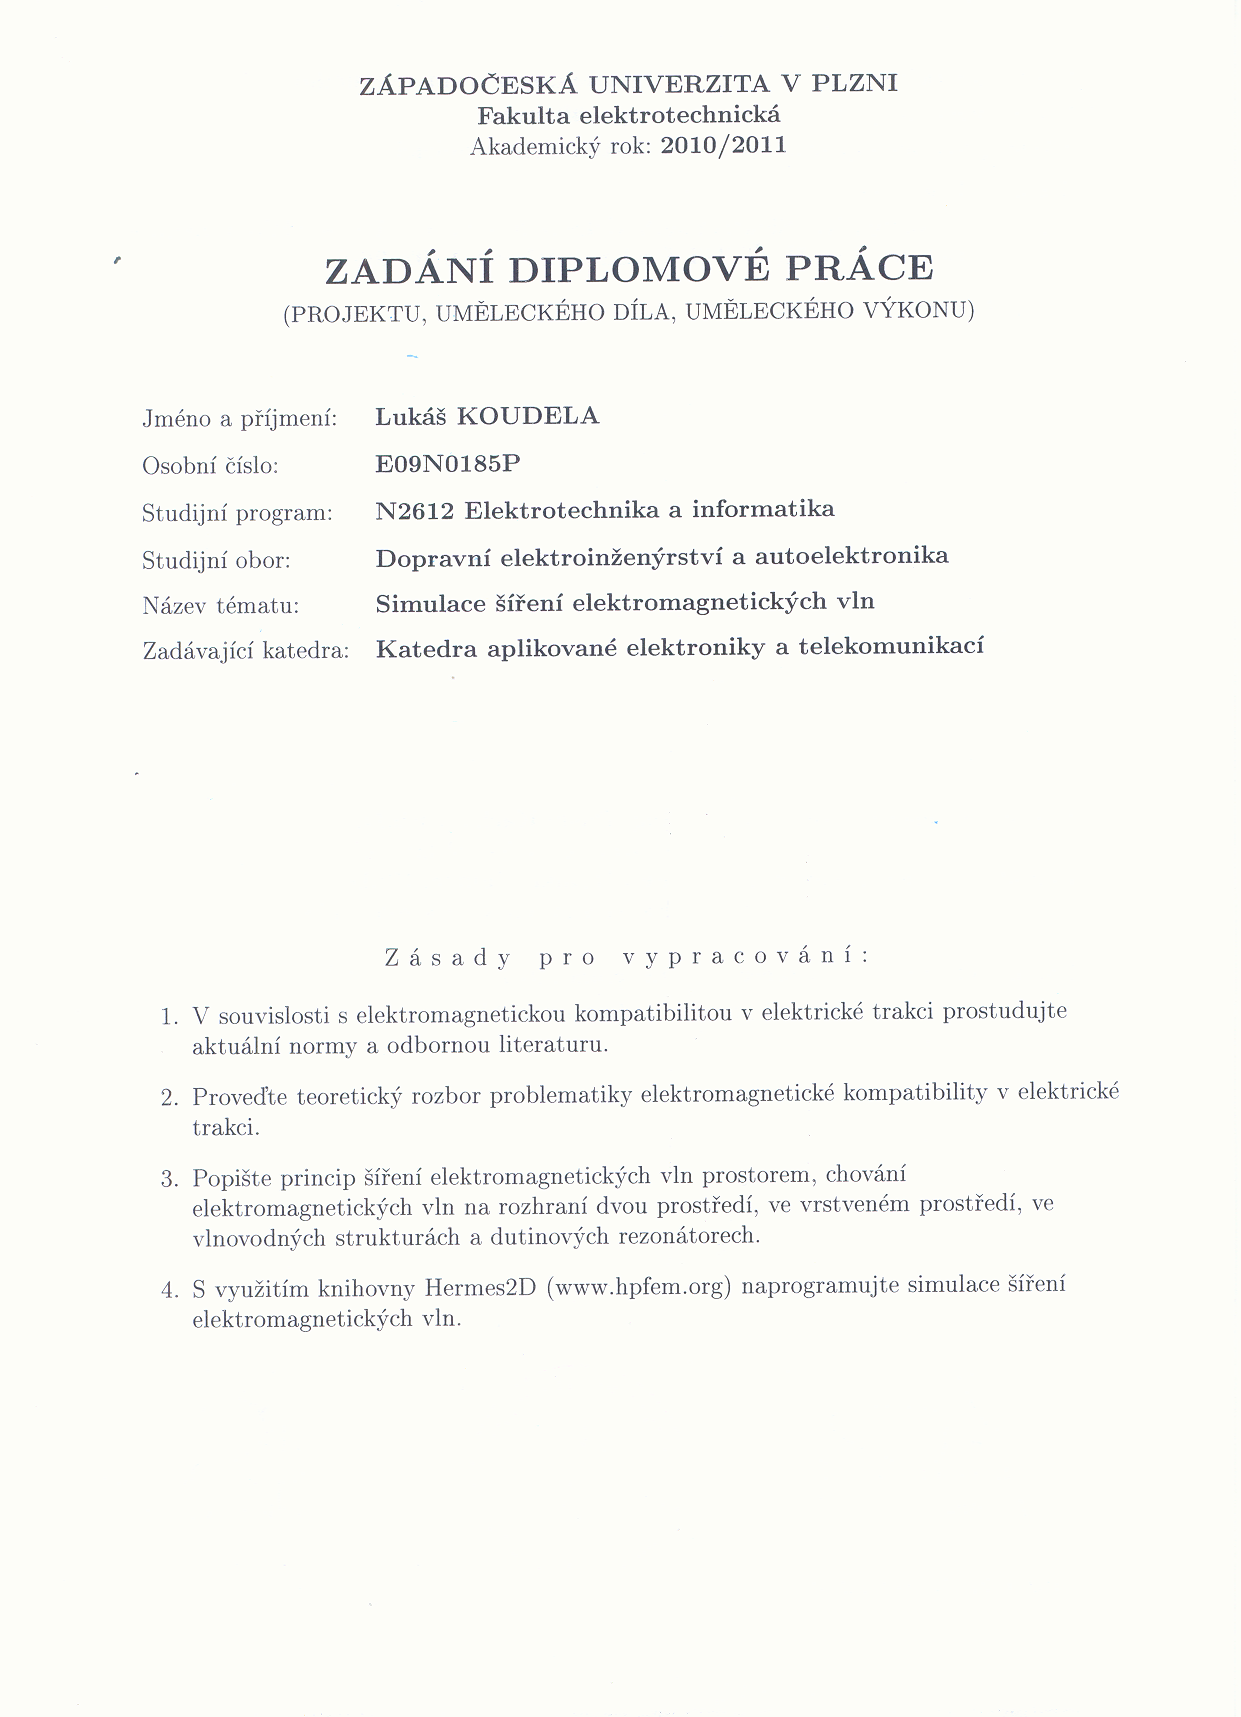
\includegraphics[width=15cm]{zadani1.png}
\end{figure}
\titlepage
\begin{figure}[!h]
	\centering
	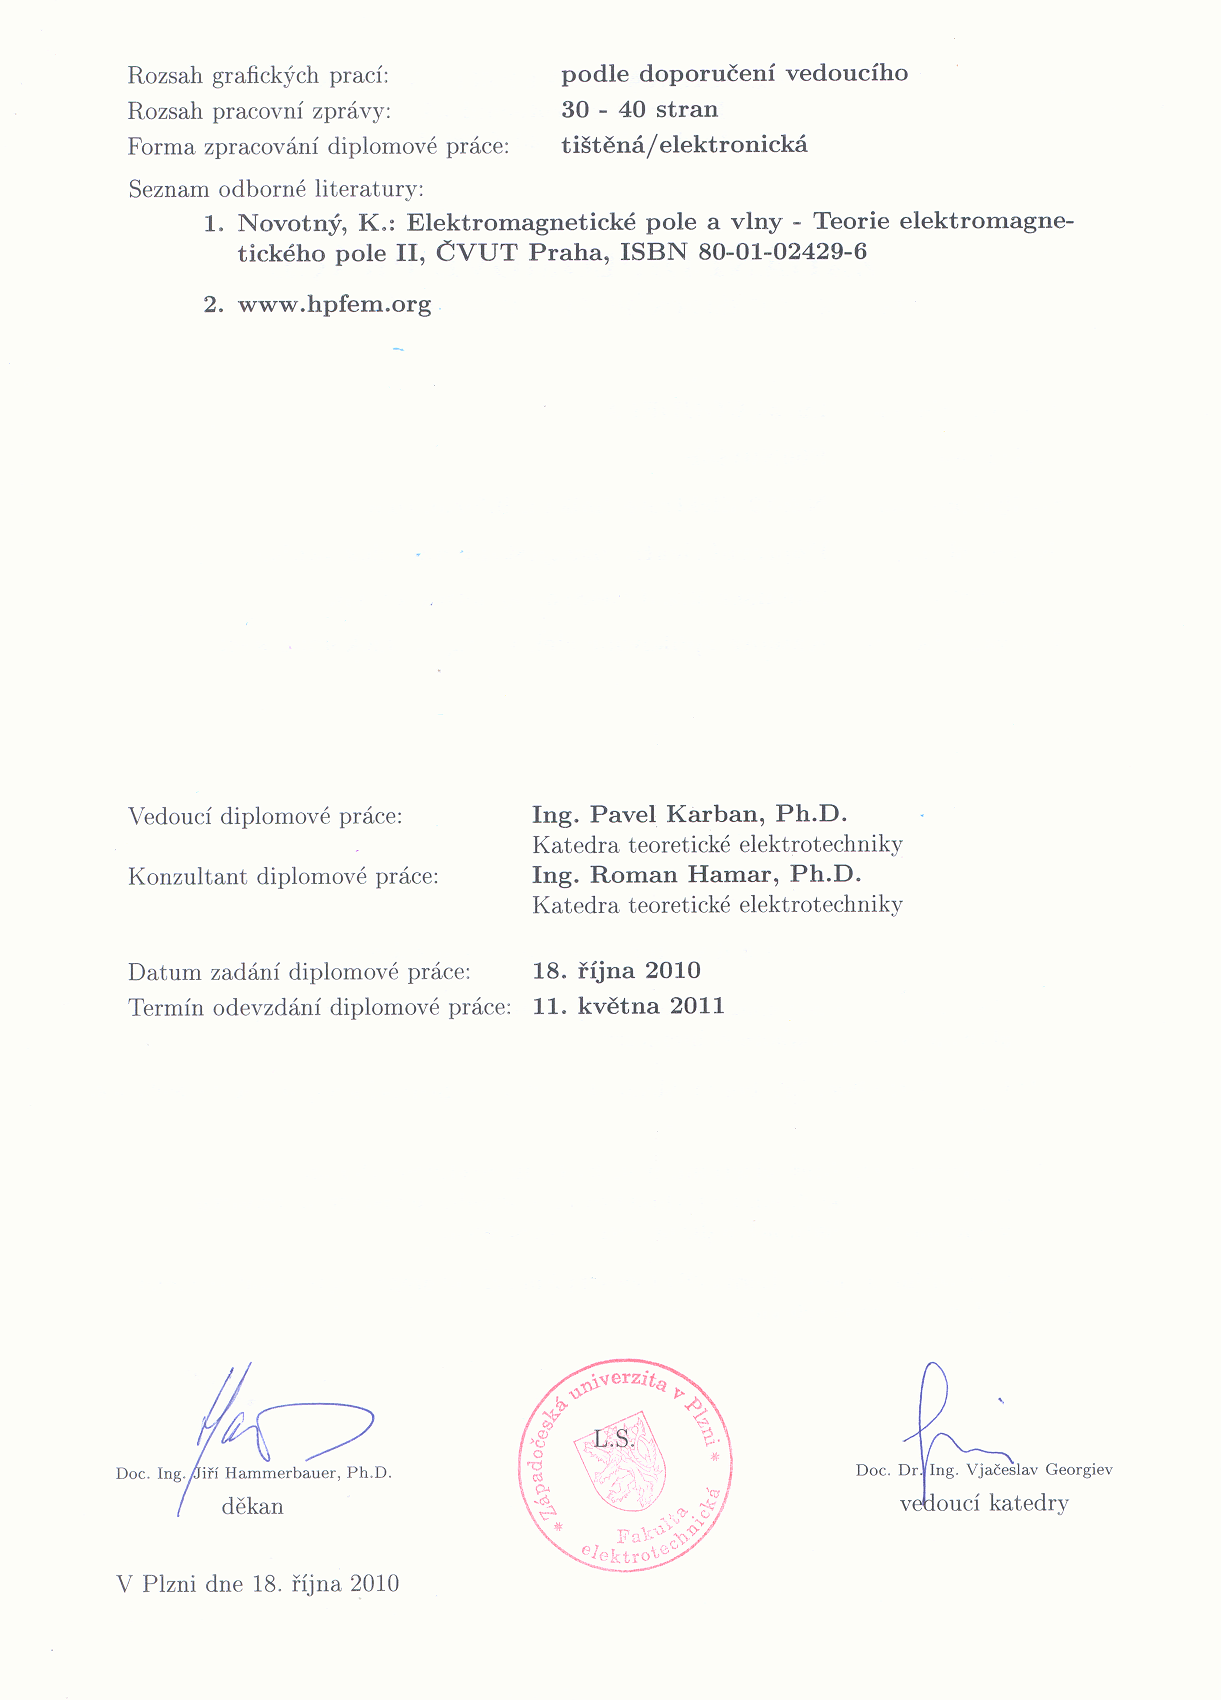
\includegraphics[width=15cm]{zadani2.png}
\end{figure}
\newpage

\section*{Anotace}
Diplomová práce se zabývá principem šíření elektromagnetických vln a jejich chování v~různých fyzikálních prostředích. Pojednává o~problematice elektromagnetické kompatibility v~elektrické trakci a uvádí související normy. Praktická část popisuje realizaci softwarové aplikace pro simulaci s~využitím knihovny Hermes2D.

\section*{Klíčová slova}
EMC, elektrická trakce, programovací jazyk C++,  Qt SDK, Hermes2D, Agros2D

\bigskip
% The Simulation of Electromagnetic Wales Propagation

\section*{Annotation}

The present thesis deals with the principle of electromagnetic waves propagation and their behavior in different physical environments. It discusses the issues of electromagnetic compatibility in electric traction and provides related standards. In the practical part, the realization of software application for simulation using the library Hermes2D is described.

\section*{Keywords}
EMC, Electric traction, programming language C++, Qt SDK, Hermes2D, Agros2D
\newpage

\section*{Prohlášení}
Předkládám tímto k~posouzení a obhajobě diplomovou práci zpracovanou na závěr studia na Fakultě elektrotechnické Západočeské univerzity v~Plzni.

\hyphenation{literatury}
Prohlašuji, že jsem diplomovou práci vypracoval samostatně s~použitím odborné literatury a pramenů uvedených v~seznamu, který je součástí této diplomové práce.
Dále prohlašuji, že veškerý software, použitý při řešení této diplomové práce, byl využit podle pravidel stanovených autorem.\bigskip \bigskip \\

\noindent V~Plzni, dne 23. dubna 2011 \hfill \ldots \ldots \ldots \ldots \ldots \ldots \ldots \ldots \ldots \ldots
\noindent \begin{flushright}Bc. Lukáš Koudela ~~~~~~~\end{flushright}
\newpage

\section*{Poděkování}
Na tomto místě bych rád vyjádřit poděkování vedoucímu diplomové práce Ing. Pavlu Karbanovi, Ph.D., a konzultantu Ing. Romanu Hamarovi, Ph.D., za veškeré cenné rady, konstruktivní připomínky, ochotu a čas, který mi při řešení problémů spojených s~touto prací věnovali.

\hyphenation{Mlsnové}
Také bych touto cestou chtěl poděkovat svým rodičům a přítelkyni Stanislavě Mlsnové za veškerou jejich nedocenitelnou podporu během studia. Bez jejich pomoci by tato práce nikdy nevznikla.\bigskip \bigskip \\

\noindent V~Plzni, dne 23. dubna 2011 \hfill \ldots \ldots \ldots \ldots \ldots \ldots \ldots \ldots \ldots \ldots
\noindent \begin{flushright}Bc. Lukáš Koudela ~~~~~~~\end{flushright}
\newpage